\section{EM Algorithm}
\label{sec:emalgorithm}

An elegant and powerful method for finding maximum likelihood parameter estimates
for probabilistic models with latent variables is the \emph{Expectation Maximization} 
	algorithm. The EM algorithm is an iterative process consisting of two
	steps: an expectation step (E-step) and a maximization step (M-step). During the iterations, a sequence of model parameters ${\bf \theta^{0}}$
, ${\bf \theta^{1}}$, ...., ${\bf \theta^{*}}$ is generated where ${\bf \theta^{0}}$ is the initial parameter and ${\bf \theta^{*}}$ is the converged parameter when the algorithm terminates. Under typical conditions, which hold in our model, the sequence of parameters guarantees monotonic improvement of the likelihood function and almost always converges to a (local) maximum-likelihood estimate.

\subsection{E-step}
\label{subsec:estep}

Suppose we have a data set of RSSI observations at
the sniffers from the target device: ${\bf \overline{S}}$ = \{
${\bf {s}}^{1}$, ${\bf {s}}^{2}$,\ldots,${\bf {s}}^{M}$\}. The E-step
corresponds to finding the expected value of the latent or hidden component ({\bf
		x} and {\bf z}) values given the observed data  ${\bf \overline{S}}$ and the current parameter estimates.
Using this observation set and the current parameter estimates, we find out the posterior probabilities (or responsibilities) as follows. \\

\noindent For each observation ${\bf {s}}^{l}$,
\begin{align}
& \pi_{(j,k)}^{l}  = p({x_{j}} = 1, {z_{k}} = 1 | {\bf{s}}^{l}) \\ 
& = \frac { p({x_{j}} = 1)p({z_{k}} = 1)p( {\bf {s}}^{l} | {x_{j}} = 1, {z_{k}} = 1)} {\ \sum_{p=1}^J \ \sum_{q=1}^{K} p({x_{p}} = 1) p({z_{q}} = 1) p( {\bf {s}}^{l} | {x_{p}} = 1, {z_{q}} = 1)} \nonumber \\ 
& = \frac { \upsilon_{j} \ \tau_{k} \mathcal{N}(\mathbf{s} |  \boldsymbol\mu_{(j,k))},\boldsymbol\sigma_{(j,k)}^2)} {\sum_{p=1}^J \sum_{q=1}^K \upsilon_{p} \tau_{q} \mathcal{N}(\mathbf{s} |  \boldsymbol\mu_{(p,q))},\boldsymbol\sigma_{(p,q)}^2) } \, . 
\end{align}

\noindent The posterior probability value $\pi_{(j,k)}^{l}$ can be viewed as the {\it responsibility} that component $(j,k)$ takes for explaining observation ${\bf {s}}^{l}$. We compute this measure of responsibility for each observation in the data set ${\bf \overline{S}}$.

\subsection{M-step}
\label{subsec:mstep}

The M-step of the algorithm corresponds to maximizing
the \emph{expected} log-likelihood of the observed data. This leads us to re-estimating the parameters for the next iteration based on the posterior probabilities calculated in the expectation step of the algorithm
\begin{align}
\upsilon_{j} = \frac { \sum_{l=1}^{M} \ \sum_{k} \pi_{(j,k)}^{l}} {M},
\end{align}
\begin{align}
\tau_{k} = \frac { \sum_{l=1}^{M} \ \sum_{j} \pi_{(j,k)}^{l}} {M},
\end{align}
\begin{align}
\mu_{i \ (j,k)} = \frac  { \sum_{l=1}^{M} \pi_{(j,k)}^{l} s_{i}^{l}} {N_{j,k}},
\end{align}
where
\begin{align}
{N_{j,k}} = \sum_{l=1}^{M} \pi_{(j,k)}^{l}.
\end{align}

The variance parameter can also be updated accordingly.

\subsection{Convergence of Log Likelihood}
\label{subsec:convergenceofloglikelihood}

\begin{figure}
\centering
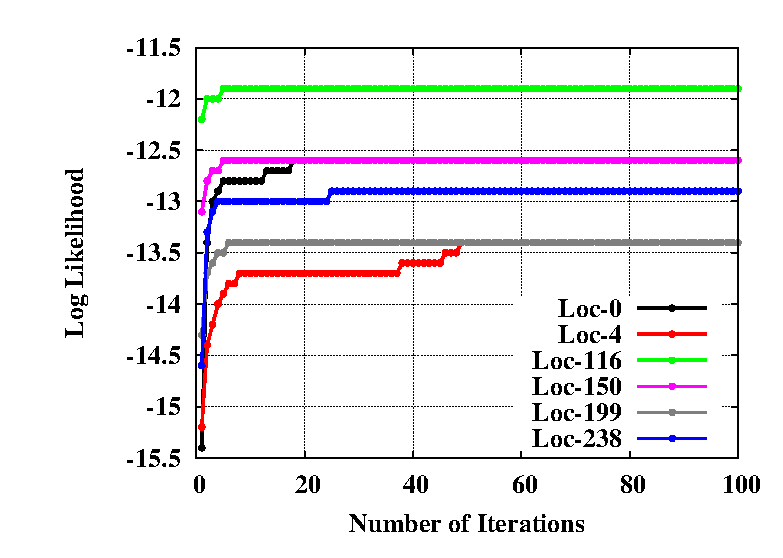
\epsfig{file=Figs4Paper/CEWIT/GMM-LogLikelihood/LogLikelihood.eps, height=1.5in, width=2.5in}
\caption{Convergence of log likelihood for 6 different instances of using WiGEM.}
\label{fig:loglikelihood}
\end{figure}

Each update of the parameters resulting from an E-step followed by an
M-step is guaranteed to increase the log likelihood function
\begin{align}
\ln p({\bf \overline{S}} | {\bf \theta}) &= \sum_{l=1}^{M} \ln \left\{
\sum_{j=1}^J \sum_{k=1}^K \upsilon_{j} \tau_{k} \mathcal{N}(\mathbf{s} |  \boldsymbol\mu_{(j,k))},\boldsymbol\sigma_{(j,k)}^2) \right\}.
\end{align}

The algorithm is deemed to have converged when the change in the log likelihood function between two successive iterations falls below a threshold ($10^{-6}$ in the experiments described later). 
Figure~\ref{fig:loglikelihood} shows how the log-likelihood converges for six different instances of running WiGEM. Each instance here is to localize an Android phone on the CEWIT testbed (Section \ref{subsec:testbeddetails}). \\ 

%Hereafter, we refer to our algorithm as {\bf WiGEM}.

\subsection{Handling Identifiability in WiGEM}
\label{subsec:handlingidentifiabilityinourmodel}

There is an identifiability problem in this general approach that is well understood~\cite{Bishop:2006:PRM:1162264}. This arises because there are $U!$ equivalent solutions
in a $U$ component mixture model. In our case,
each component is a (location,
power-level) pair. 
We handle the problem of identifiability 
by using the knowledge of sniffer locations to initialize the EM algorithm
using the basic log-distance radio propagation model~\cite{Rappaport:2001:WCP:559977, Molkdar91} below :
%\subsubsection{Indoor Radio Propagation Model}
%\label{subsubsec:indoorradiopropagationmodel}
\begin{align}
P_r(d) = G\frac{P_t}{d^\alpha},
\end{align}
where $P_r(d)$ is the received power at distance $d$ and $P_t$ is the transmit power.
$\alpha$ is the path loss exponent which is simply a model parameter. 
In free space $\alpha =2$, but it typically increases somewhat in complex 
environments. $G$ is a frequency and antenna dependent constant. 
Often the above equation is expressed somewhat differently as 
\begin{align}
P_r(d) = P_r({d_0}) - 10\alpha\log\left(\frac {\it d} {\it d_{0}}\right)
	\label{eqn:pathloss_1},
\end{align}
%\noindent
where $P_r$ is now expressed in decibel (dB) units. This emphasizes that when powers 
are expressed in dB units transmit power changes expressed in dB cause the same dB change at all receivers
regardless of location. In our experiments we will use RSSI in dB units. We independently
verified (not reported here for brevity) that the RSS measurement on our sniffer hardware is accurate at least to the extent
that a dB shift in the transmit power does get recorded as a similar
shift at the sniffer regardless of location.

%\subsubsection{Reference Signal Power and the Path Loss Parameter}
%\label{subsubsec:referencesignalpathloss}
%
%In Equation \ref{eqn:pathloss_1},  $P_r({d_0})$ is the signal power at
%some reference distance $d_{0}$ from the sniffer. This reference signal
%strength $P_r({d_0})$ can be derived empirically or obtained from
%wireless network hardware specifications \cite{Bahl00radar:an}. In our
%deployment all our sniffers have the same hardware (described in detail
%		in Section \ref {sec:evaluation}) . The value of $P_r({d_0})$
%was empirically found to be approximately 60 dB when $d_{0}$ = 1 meter . No assumption is made about the
%target space, so $\alpha =2$. The path loss equation of equation
%\ref{eqn:pathloss_1} can now be succintly expressed as 
%\begin{align}
%P_r(d) = 60 - 10\alpha\log\left({\it d} \right)  .
%	\label{eqn:pathloss_2}
%\end{align}

\subsubsection{Initializing the Model Parameters}
\label{subsubsec:initializingthecomponentsofourmodel}

\begin{itemize}

\item ${\boldsymbol\upsilon}$ and ${\boldsymbol\tau}$ are initialized as being from a uniform distribution over locations and power levels respectively.

\item For a location $l_{j}$, Equation \ref{eqn:pathloss_1} gives us the theoretical RSSI value  $w_{ij}$ (say) at a sniffer $s_{i}$. The reference power $P_r({d_0})$
is assumed to be 60 (in dB units) at $d_0=1$ meter. Note that the reference power
assumption is somewhat arbitrary. The parameter $\alpha$ is assumed to be 2. 

We consider $K$ values reflecting the power levels:
\begin{align}
\left\{ (w_{ij}-\frac{K}{2}), (w_{ij}-\frac{K}{2}+1), \dots ,(w_{ij}+\frac{K}{2})\right\}. \nonumber
\end{align}
The values are used to initialize the means, $\mu_{i, (j,k)}$ of the $K$ components corresponding to location $l_{j}$ and sniffer $s_{i}$. We do this for every target location in the map and for each sniffer in the building. This effectively initializes parameter ${\boldsymbol\mu}$ in WiGMM. 

Note: negative values are not allowed and are set to 0 during initialization.

\item The standard deviation parameter, ${\boldsymbol\sigma}$, is initialized to 5 for each component in WiGMM (and kept fixed to reduce computation time). This choice is mostly arbitrary. Some previous work \cite{Tao:2003:WLL:941311.941314} also use fixed values of standard deviation ($\sigma=12$) in their work. \\

\end{itemize}

%, that should be observed at the
%sniffer for a client transmitting from $l_{i}$. 

% However, different devices may work at different power-levels
% for doing wireless transmissions. To handle this scenario, we consider $K$ values for each location $l_{i}$:
% \begin{align}
% \{ (w_{i}-\frac{K}{2}), (w_{i}-\frac{K}{2}+1), \dots ,(w_{i}+\frac{K}{2})\}.
% \end{align}
% Use these values to initialize the means for the $K$ different
% components corresponding to location $l_{i}$. Recall from Section \ref{subsec:latentvariablesfortargetlocationsandpowerlevels}, that WiGMM has a $K$-dimensional binary random variable $\mathbf{z}$ representing Power Levels.     {\bf We do this procedure for every possible
% target location in the map, so that we initialize the mean of every component in WiGMM}.  The standard deviation ($\sigma_{j, k}$)
% 	was chosen as 5 (and kept fixed to reduce computation time). This
% 	choice was mostly arbitrary though some previous work
% 	\cite{Tao:2003:WLL:941311.941314} also use fixed values of standard
% 	deviation ($\sigma=12$) in
% 	their work. 

\subsection{Final Location Estimate}
\label{subsec:finallocationestimate}

\begin{figure}
	\centering
		\subfloat[CEWIT]{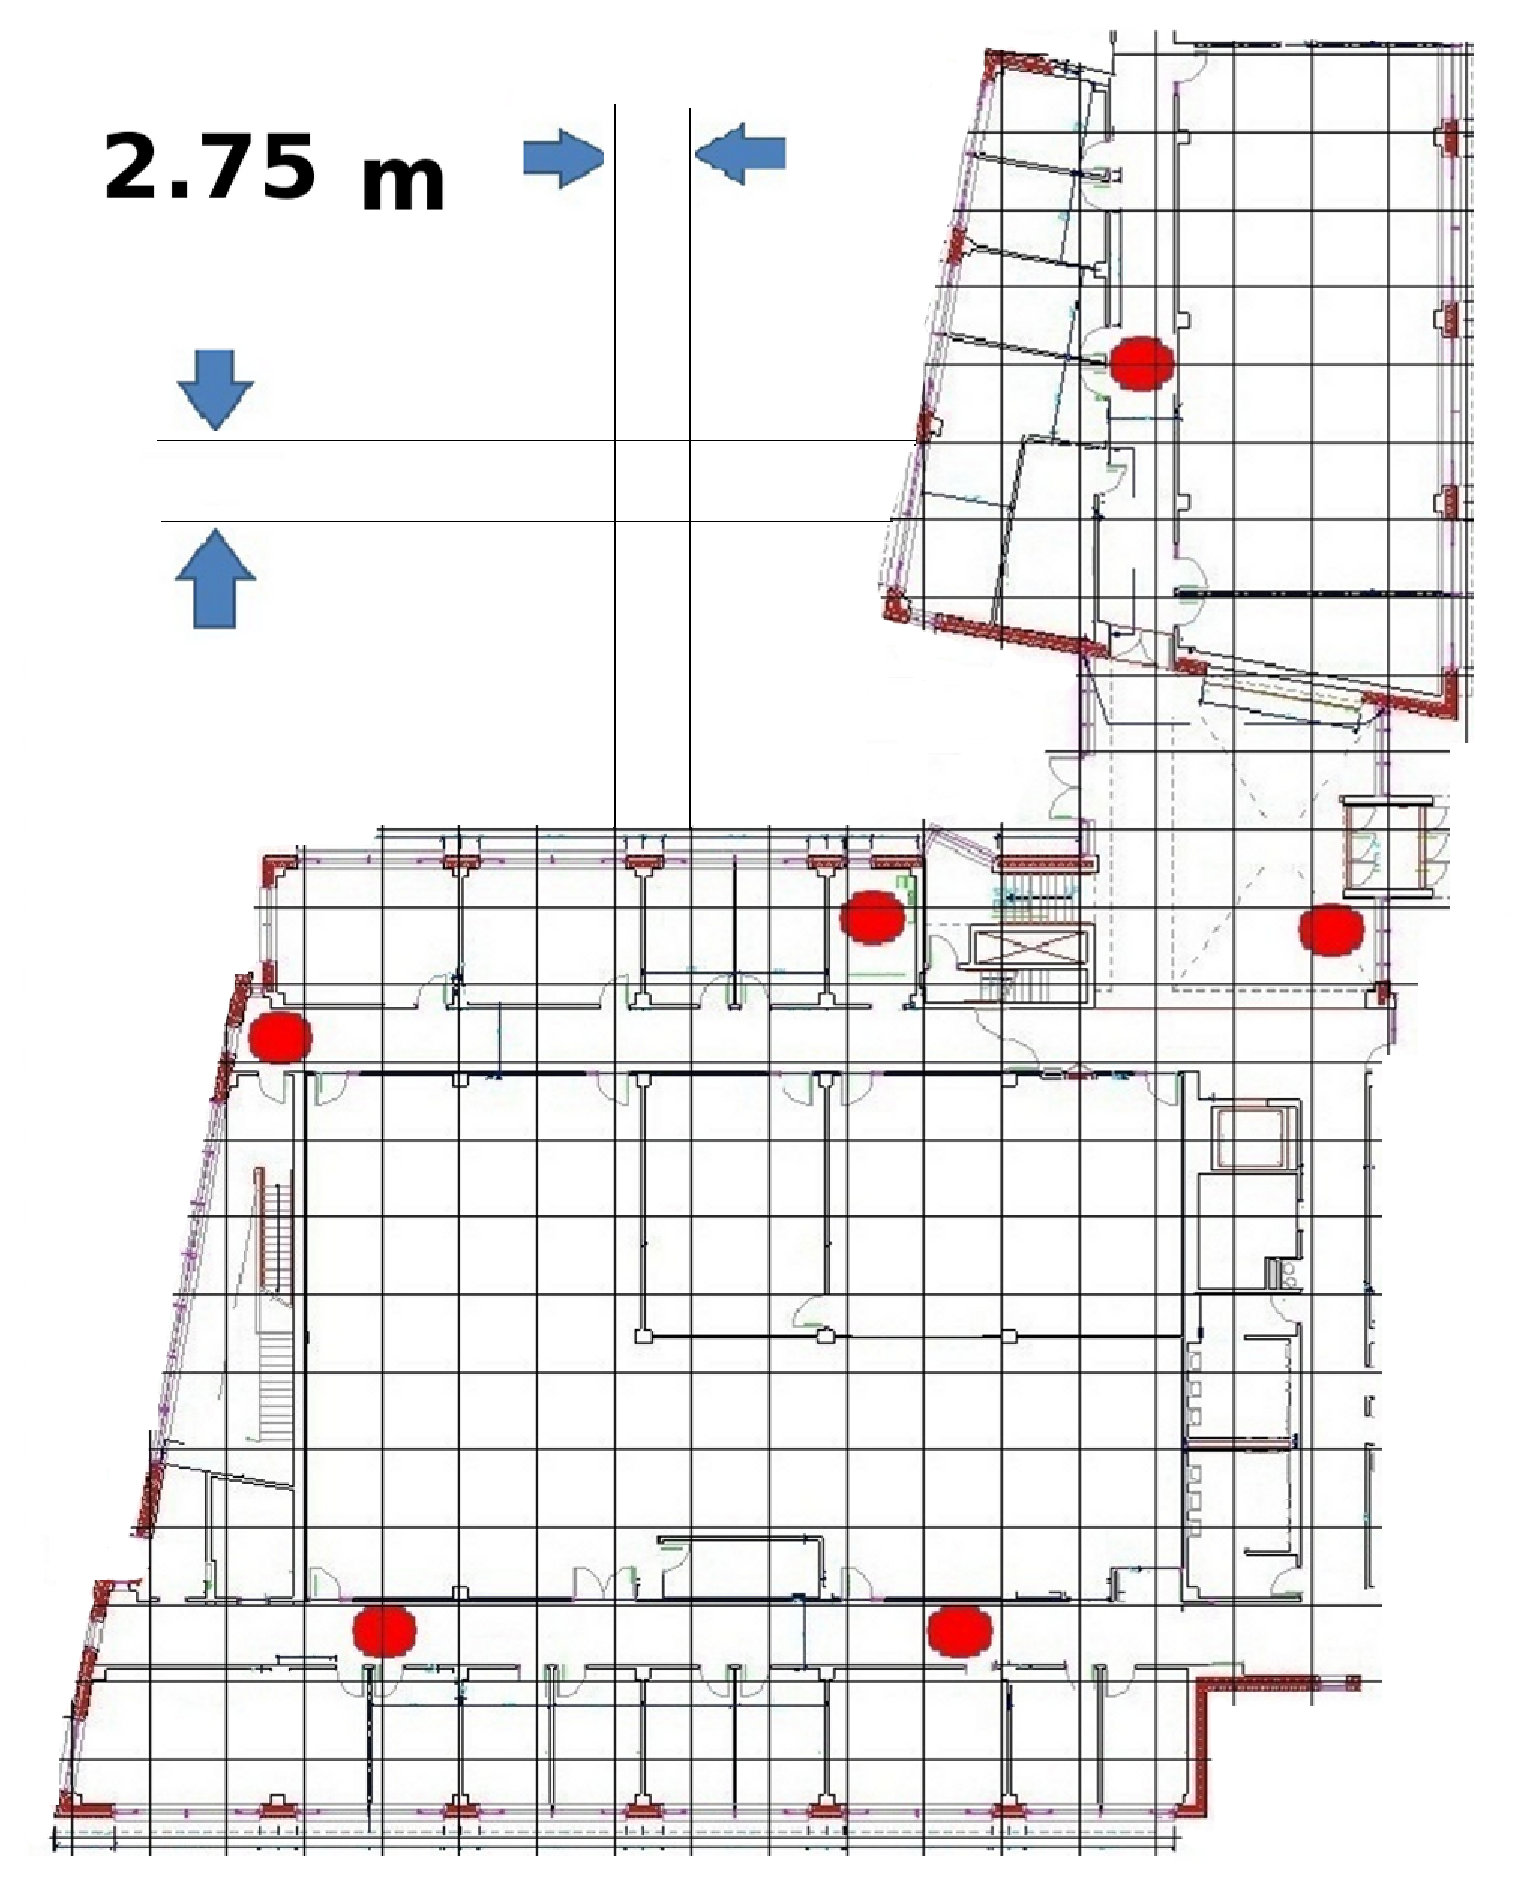
\includegraphics[height=1.8in]{Figs4Paper/CEWIT/CEWIT-Map7.eps}} \quad \quad \\
		\subfloat[CSD]{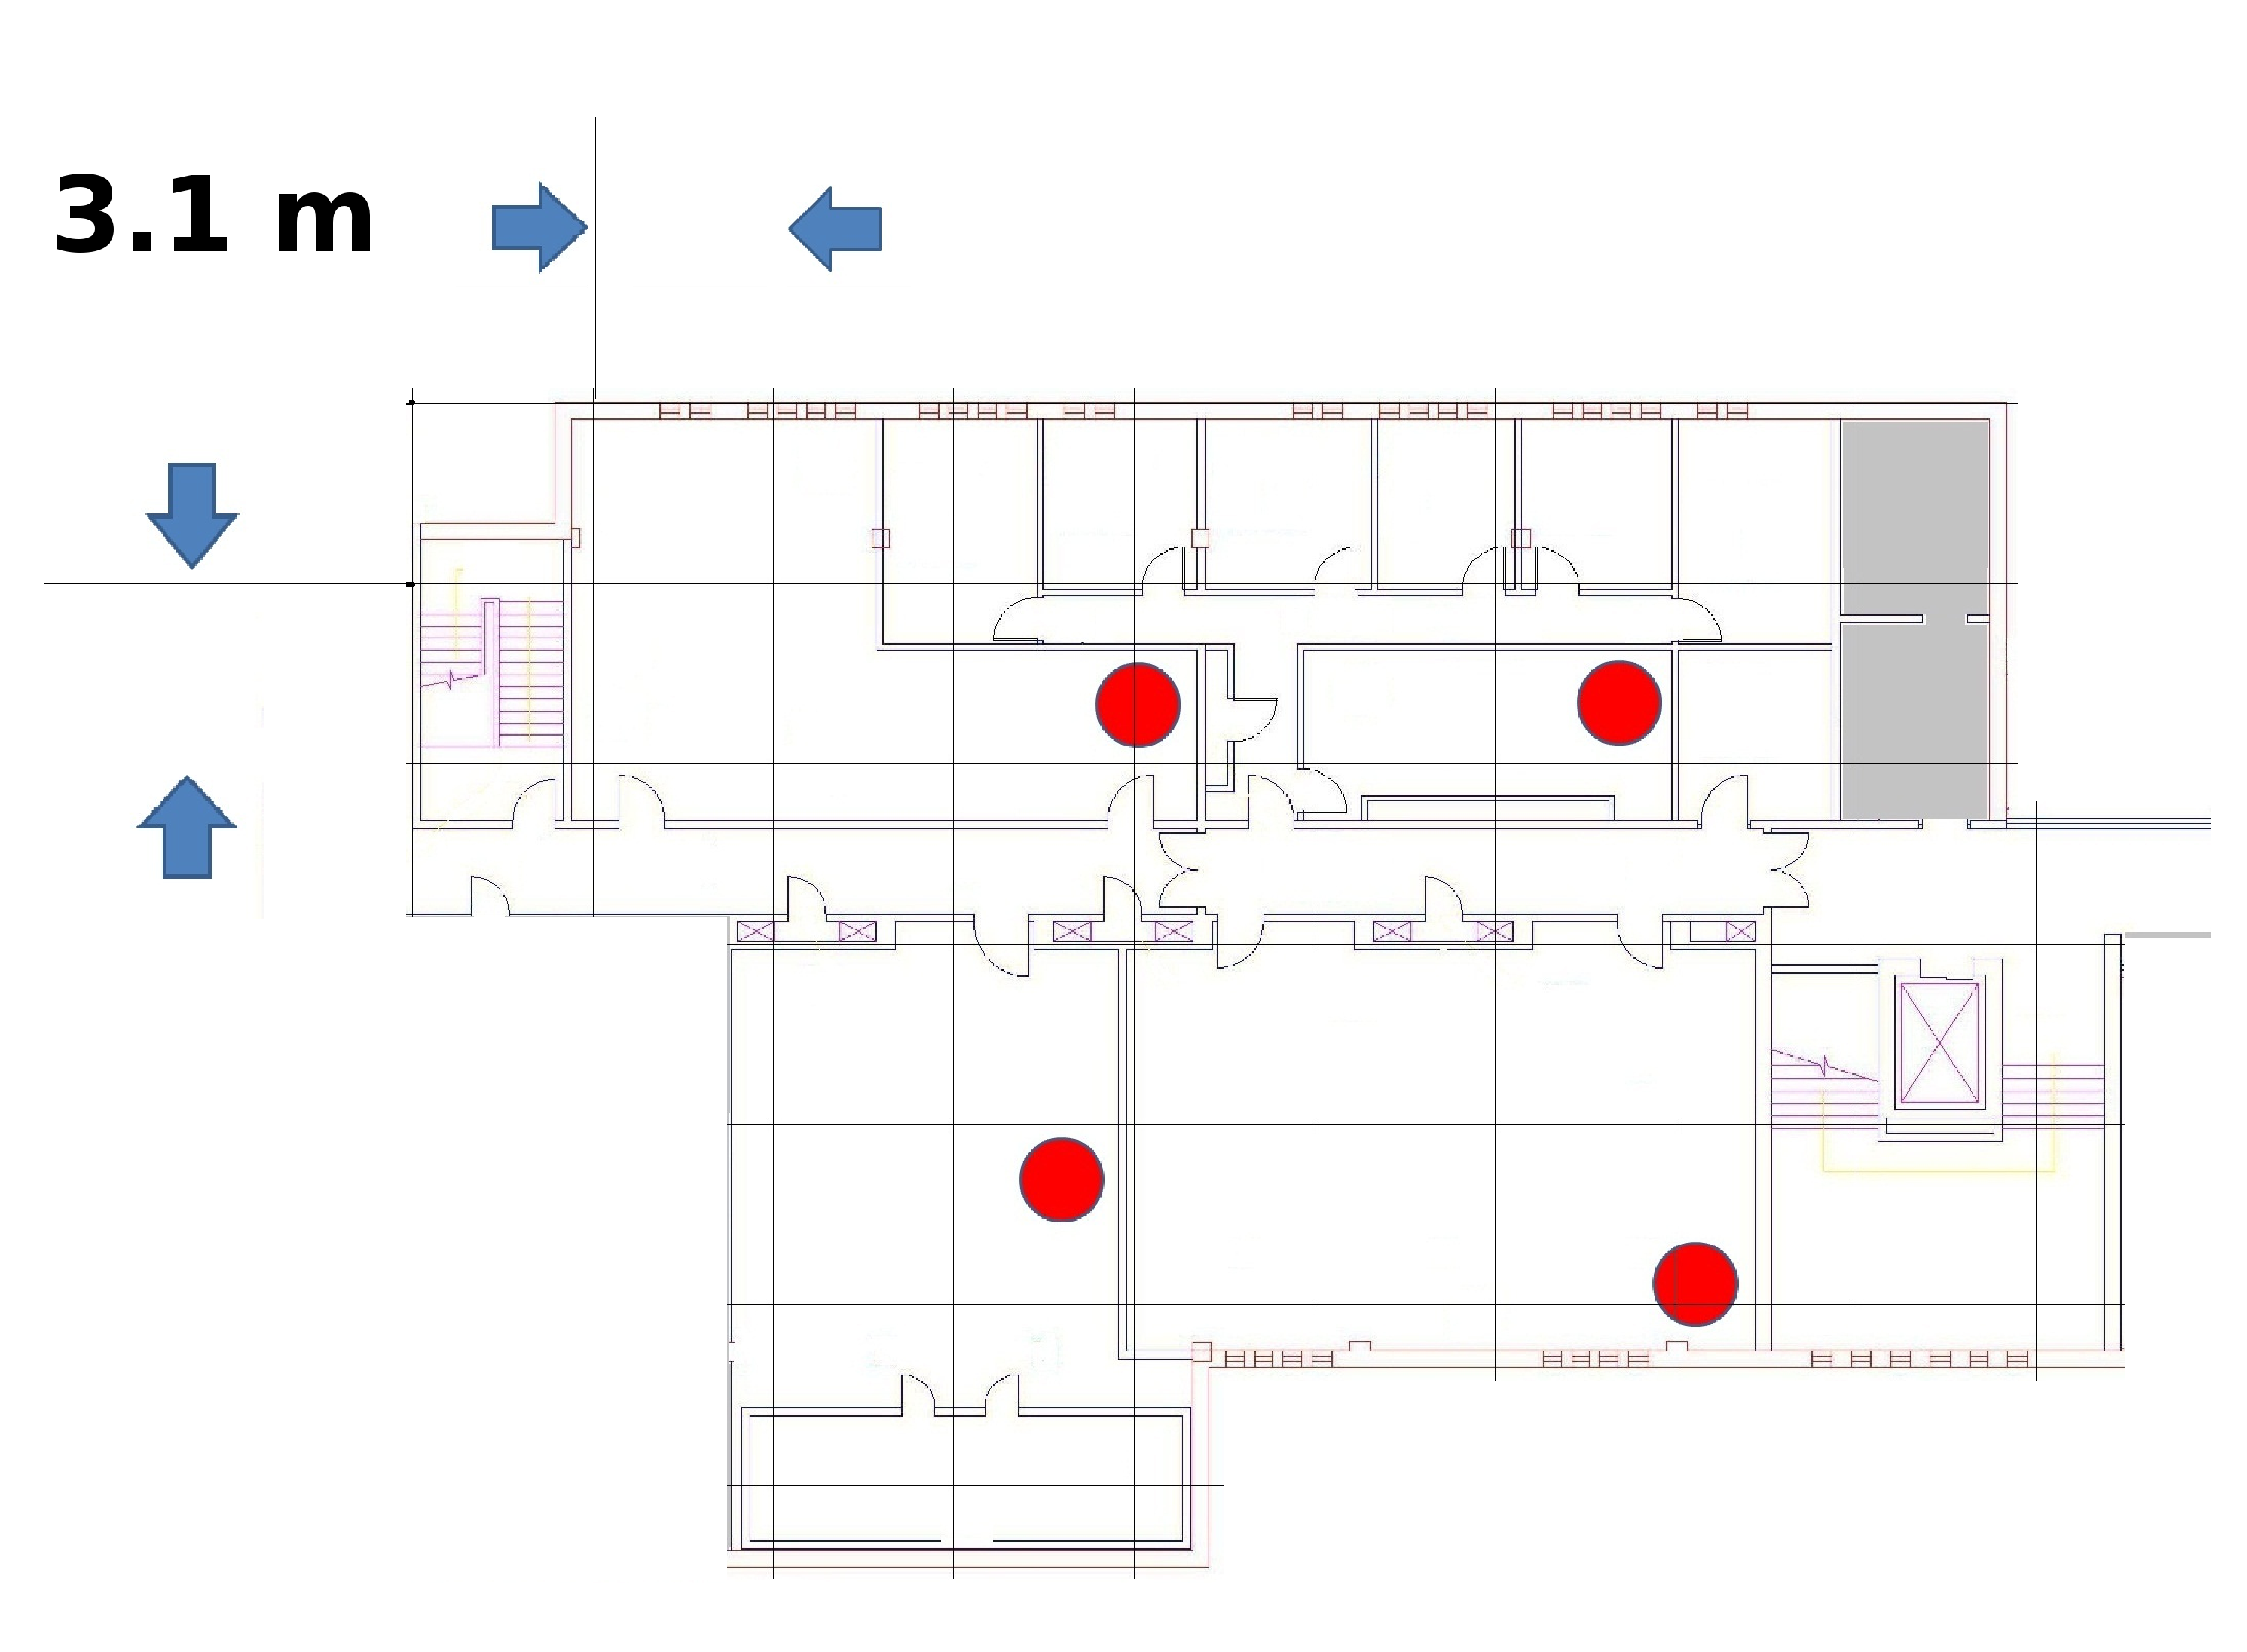
\includegraphics[width=2in]{Figs4Paper/CSD/CSD-Map4.eps}} 
	\caption{Two testbeds for validation experiments. The finer grids are 
	shown (see text). The red circles represent sniffer locations.}
	\label{fig:experimenttestbed}
\end{figure}


Given a real-time received RSSI vector ${\bf {s}}^{(obs)}$, we can now
find the location with the highest probability. We do this by first
finding the probability for each (location, power-level) pair and then
marginalizing over the power-levels. This gives us a probability
distribution over the possible locations inside the target space. The
location with the highest probability is returned as the answer.
Thus the estimated location index is given by $j^{*}$, where
\begin{align}
j^{*} = \arg\max_{j} \sum_{k} p({x_{j}} = 1, {z_{k}} = 1 | {\bf {s}}^{(obs)}) \, .
\end{align}
